\section{Ejercicio 1}

\subsection{Introducción}

\paragraph{}
El primer problema de este trabajo práctico consistió en dar un algoritmo que sea capaz de decir, dada una secuencia de números, la mínima cantidad de números a eliminar de la misma para que ésta sea unimodal. Esto es, que la secuencia cumple que es creciente desde el primer elemento hasta cierta posición y desde dicha posición es decreciente hasta el final\footnote{Debe ser estrictamente creciente/decreciente}.

\paragraph{}
Además, se estableció como requerimiento que la complejidad del algoritmo en cuestión fuera estrictamente menor que \Ode{n^3}, siendo n el tamaño de la secuencia.

\paragraph{}
Se pensaron varias formas de encarar y resolver este problema, finalmente se aplicó la técnica de \textit{programación dinámica}. En las sucesivas secciones, daremos una explicación detallada de cómo se implementó el algoritmo, cuál es su complejidad temporal y cómo se comportó frente a distintos valores y tamaños de entrada.


\subsection{Explicación}

\paragraph{}
Desde un comienzo se pensó que el problema podía resolverse usando \textit{programación dinámica}, sin embargo comprender de qué forma debía aplicarse \textit{principio de optimalidad} no fue, en principio, nada trivial. Tras un tiempo de analizar el problema, se pudo vislumbrar que el mismo podía ser visto como una variación de otro problema similar: el de encontrar dentro de una secuencia la subsecuencia creciente/decreciente más larga. \\
Básicamente, el razonamiento empleado fue el siguiente:\\

Si para cada posición \textit{i} de la secuencia se conoce:
\begin{itemize}
	\item Longitud de la subsecuencia creciente más larga desde el principio hasta \textit{i} (que contenga al elemento i-ésimo)
	\item Longitud de la subsecuencia decreciente más larga desde \textit{i} hasta el final (que contenga al elemento i-ésimo)
\end{itemize}

entonces es posible decir cuál es el largo de una secuencia unimodal que tiene como ``pivote'' u objeto más grande al i-ésimo de la secuencia. Finalmente, sólo bastaría averiguar cuál es el ``pivote'' que maximice esa longitud para de ésta forma resolver el problema.\\
\textbf{Cabe observar, que determinar la longitud de la subsecuencia unimodal más larga es equivalente a encontrar la cantidad mínima de elementos a eliminar para transformar la secuencia dada en una secuencia unimodal. Este dado será tenido en cuenta a la hora de implementar el algoritmo.}

\paragraph{}
A continuación se desarrolla el funcionamiento del algoritmo mediante el cual se logra resolver el problema planteado.\\

Para construir el algoritmo de programación dinámica se definieron:
\begin{itemize}
	\item un vector denominado \textit{ascenso} donde se va guardando, en la i-ésima posicion, la longitud de la subsecuencia más larga desde el inicio de la secuencia original hasta la posición i. Esto es: \\ $ascenso_i$ = longitud de la secuencia creciente más larga que termina con el número $v_i$
	\item la siguiente relación de recurrencia:	 
	\begin{itemize} 
		\item $ascenso_0 = 0$
		\item $ascenso_i  = max_{j<i} \left\lbrace ascenso_j + 1\right\rbrace  \;      $ (con $ v_j < v_i  $)
	\end{itemize}
	\item y la solucion final: $max_{1\leq i\leq n} \{ascenso_i\}$
\end{itemize}

\paragraph{}
Para entender el algoritmo principal, se presenta el pseudocódigo de la función \textit{completar\_ascensos}, la cual completa el vector \textit{ascenso} con los valores correspondientes.

\incmargin{1em}
\linesnumbered
\restylealgo{boxed}

\begin{algorithm}[H]
	void  \textbf{completar\_ascensos}(ascenso: vector$<nat>$, v: vector$<int>$)\\
	\BlankLine		
	\BlankLine		
	\SetKw{Orden}{Complejidad:}
	\Orden{$\theta$($tam(v)^2$)}
	\BlankLine		


    \For{($i = 0;i<= tam(v);i++$)\tcp*{$\theta(tam(v)^2))$ \ \ \footnote{esta complejidad se da ya que $\displaystyle\sum_{i=0}^{tam(v)} (i)  = \frac{tam(v)*(tam(v)-1)}{2} \in \theta(tam(v)^2)$}}}{ascenso[i] $\leftarrow$ maximoAsc(ascenso,v,i) + 1\tcp*{$\theta$($i$)}}
\end{algorithm}
	

\paragraph{}
La función maximoAsc(ascenso,v,i) indica, dentro del vector ascenso, la maxima longitud de un ascenso hasta la posicion i-1 del vector tal que cumpla la siguiente propiedad:

\vspace*{1cm}

Si j es el indice del ascenso donde se encuentra el resultado, tiene que ocurrir que: \footnote{ver pseudocódigo en el anexo}

$$(\forall k \in [0...i) , v[k]<v[i]) \  ascenso[j] > ascenso[k]$$


Por lo tanto, de esta manera podemos obtener para cada pivote, la longitud del mayor ascenso hasta esa posición.

\vspace*{1cm}
Veamos un \textit{ejemplo}:

$v = \left\lbrace 9,5,2,8,7,3,1,6,4\right\rbrace$ 

Las subsecuencias ascendentes más largas son $\left\lbrace 2,3,4\right\rbrace$ o $\left\lbrace 2,3,6\right\rbrace$

\begin{center}
   \begin{tabular}{| l | c | c |c |c |c |c |c |c |c | }
     \hline
     sucesión & 9 & 5 & 2 & 8 & 7 & 3 & 1 & 6 & 4 \\ \hline
     longitud & 1& 1& 1& 2& 2& 2& 1 &3 & 3 \\ \hline
     
     \hline
   \end{tabular}
 \end{center}

Aquí podemos observar que en cada posición de la fila longitud, se encuentra la longitud de la secuencia creciente más larga hasta ese punto.

\paragraph{}
Una vez realizado este proceso, podemos obtener, ejecutando un algoritmo equivalente (pero desde el final hacia el principio) que obtenga, para cada posición, la longitud de la secuencia decreciente más larga desde la posición hacia el final. Al ejecutar esté proceso sobre el ejemplo obtendríamos:

\begin{center}
   \begin{tabular}{| l | c | c |c |c |c |c |c |c |c | }
     \hline
     sucesión & 9 & 5 & 2 & 8 & 7 & 3 & 1 & 6 & 4 \\ \hline
     ascendente & 1& 1& 1& 2& 2& 2& 1 &3 & 3 \\ \hline
     descendente & 5& 3& 2& 4& 3& 2& 1 &2 & 1 \\ \hline
          \hline
   \end{tabular}
 \end{center}

Luego, para decidir cual es el mejor pivot, nos basamos en dos filas extra implicitas que podemos ver a continuación :

\begin{center}
   \begin{tabular}{| l | c | c |c |c |c |c |c |c |c | }
     \hline
     sucesión 		& 9& 5& 2& 8& 7& 3& 1 &6 & 4 \\ \hline
     ascendente 	& 1& 1& 1& 2& 2& 2& 1 &3 & 3 \\ \hline
     descendente 	& 5& 3& 2& 4& 3& 2& 1 &2 & 1 \\ \hline
     suma	 	& 5& 3& 2& 5& 4& 3& 1 &4 & 3 \\ \hline
     tam(S) - suma;	& 4& 6& 7& 4& 5& 6& 8 &5 & 6 \\ \hline
     
          \hline
   \end{tabular}
 \end{center}


\paragraph{}
Donde $suma_i = ascendente_i + descendente_i - 1 \; \forall i \in [ 1..tam(s)]$ \\(esto quiere decir, la suma de las longitudes de la secuencia de mayor longitud creciente hasta i + la longitud de la secuencia de mayor longitud decreciente desde i). Se le resta 1 porque ambas secuencias incluyen al elemento de la posición i.

La fila tam(S)-suma representa, cuantos elementos NO fueron usados para esta ``escalera''. 


\paragraph{}
Por lo tanto se busca el máximo valor de la fila suma, lo que es equivalente a buscar el mínimo en la fila tam(s)-suma que representa la cantidad minima de borrados a realizar para lograr formar la secuencia unimodal y ese es el resultado devuelto por nuestra función.


\subsection{Análisis de la complejidad del algoritmo}

\paragraph{}
A continuación se calculará la complejidad del algortimo implementado en la función \textit{escalerar}, que es el que resuelve el problema que se planteo. Primero veamos el pseudocódigo de la función completa:

\vspace*{30pt}
void \textbf{escalerar}(v: vector$\langle$int$\rangle$)\\
\SetKw{Orden}{Complejidad:}
	\begin{algorithm}[H]
	\Orden{$\theta$($tam(v)^2$)} 
\BlankLine		
      \textbf{var} max: nat;\\
      \textbf{var} ascenso: vector$\langle$nat$\rangle$(tam(v))\tcp*{$\theta$($tam(v)$)}
      \textbf{var} descenso: vector$\langle$nat$\rangle$(tam(v))\tcp*{$\theta$($tam(v)$)}
\BlankLine		
      completar\_ascensos(ascenso,v)\tcp*{$\theta$($tam(v)^2$)}
      completar\_descensos(descenso,v)\tcp*{$\theta$($tam(v)^2$)}	
\BlankLine		
      \For{($i = 0;i \leq tam(v);i++$) \tcp*{$\theta$($tam(v)$)}}{
	\lIf{(ascenso[i] $+$ descenso[i] $\geq$ max)} {max $\leftarrow$ ascenso[i] $+$ descenso[i]\tcp*{$\theta$(1)}}	
	} 
\BlankLine		
	retornar  tam(v) $-$ max $+$ 1\tcp*{$\theta$(1)}	



\end{algorithm}


\vspace*{1cm}
Pseudocódigo de la función completar\_descensos:
\\
\\

void \textbf{completar\_descensos}(descenso: vector$\langle$nat$\rangle$, v: vector$\langle$int$\rangle$)\\
\SetKw{Orden}{Complejidad:}
	\begin{algorithm}[H]
	\Orden{$\theta$($tam(v)^2$)}
\BlankLine		
     \For{($i = tam(v);i \geq 0;i--$) \tcp*{$\theta(tam(v)^2)$ \ \ \footnote{esta complejidad se da ya que $\displaystyle\sum_{i=tam(v)}^0 (tam(v) - i)  = \displaystyle\sum_{i=0}^{tam(v)} (i)  = \frac{tam(v)*(tam(v)-1)}{2} \in \theta(tam(v)^2)$}}}
     {descenso[i] $\leftarrow$ maximoDes(descenso,v,i) + 1\tcp*{$\theta$($tam(v) - i$)}}
  \end{algorithm}

\vspace*{1cm}
Pseudocódigo de la función maximoAsc:
\\
\\
nat  \textbf{maximoAsc}(ascenso: vector$\langle$nat$\rangle$, v: vector$\langle$int$\rangle$,i: nat)\\
\SetKw{Orden}{Complejidad:}
	\begin{algorithm}[H]
	\Orden{$\theta$($i$)}
	\BlankLine		
      \textbf{var} res: nat \tcp*{$\theta$(1)}
      res $\leftarrow$ 0 \tcp*{$\theta$(1)}
	\BlankLine		
     \For{($k = 0;k < i;k++$)\tcp*{$\theta$($i$)}}{
  \lIf{(v[j] $<$ v[i] and res $<$ ascenso[j])}{res$\leftarrow$ascenso[j]}\tcp*{$\theta$(1)}}
  \end{algorithm}

\vspace*{1cm}

\paragraph{}
\underline{Aclaración:} el pseudocódigo de la función competar\_ascensos() se encuentra en la sección ``Explicación'' y la función maximoDes() es analoga a maximoAsc().

\paragraph{}
Como se ve en los pseudocódigos, sin depender de los valores ingresados en el vector v, la cantidad de operaciones es la misma para un mismo tamaño de entrada. Por lo tanto, podemos decir que esta función esta acotada por arriba y por abajo por una función cuadratica a partir de un $n_0$ es decir, escalerar() $\in \titade{tam(v)^2}$

\paragraph{}
En conclusión, nuestro algoritmo esta siempre acotado por arriba y por abajo por una función cuadratica en el tamaño de la entrada (tam(v)).



\subsection{Detalles de implementación}

\paragraph{}
Para compilar el programa sólo hace falta ejecutar el comando make en consola.

\paragraph{Modo de Uso}


\pagebreak[4]
\clearpage

\subsection{Resultados}
\label{resultadosej1}

\paragraph{}
Para poder analizar el comportamiento del algoritmo, se desarrolló un generador de secuencias de tamaños determinados con valores enteros en un rango determinado.

\paragraph{}
Al realizar el análisis sobre la complejidad del algoritmo, notamos que sin importar los valores en la secuencia ni la cantidad de elementos a sacar para convertirla en unimodal, debería comportarse de manera identica para tamaños de secuencia similares.

\paragraph{}
Por lo tanto, veamos que entradas generamos:
\begin{enumerate}
  \item 100 secuencias de tamaños desde 1 hasta 99 con elementos aleatorios entre -1000000 y 1000000.
  \item 250 secuencias de tamaños desde 1 hasta 250 con elementos aleatorios entre -1000000 y 1000000.
  \item 250 secuencias de tamaños desde 1 hasta 250 con elementos iguales a cero, de manera que el resultado sea eliminar todos menos un elemento para convertirla en unimodal.
\end{enumerate}



\paragraph{}
Luego, se desprenden algunas hipótesis, las cuales enunciaremos a continuación:
\begin{itemize}
  
  \item La cantidad de operaciones no debería ser afectada por la cantidad de elementos a borrar para convertir la secuencia.

  \item Para tamaños de entradas identicos, el algoritmo debería realizar exactamente la misma cantidad de operaciones.

\end{itemize}




\paragraph{}
A continuación veremos gráficos que muestran el comportamiento del algoritmo utilizado

\newpage
	\begin{table}[h!] %ubicacion de la tabla
		\centering %centra la tabla
			\begin{tabular}{c}
				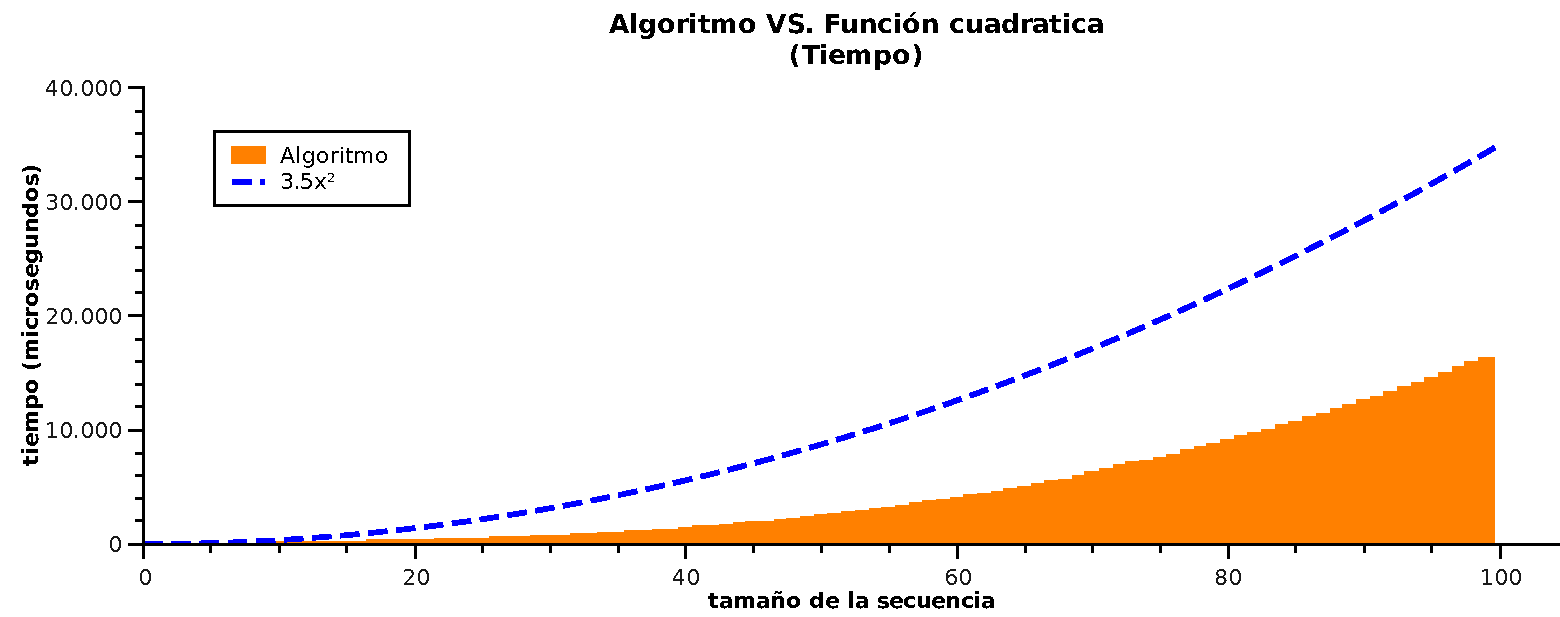
\includegraphics[scale=0.7]{../ej1/graficos/tiempo100.pdf} \\
				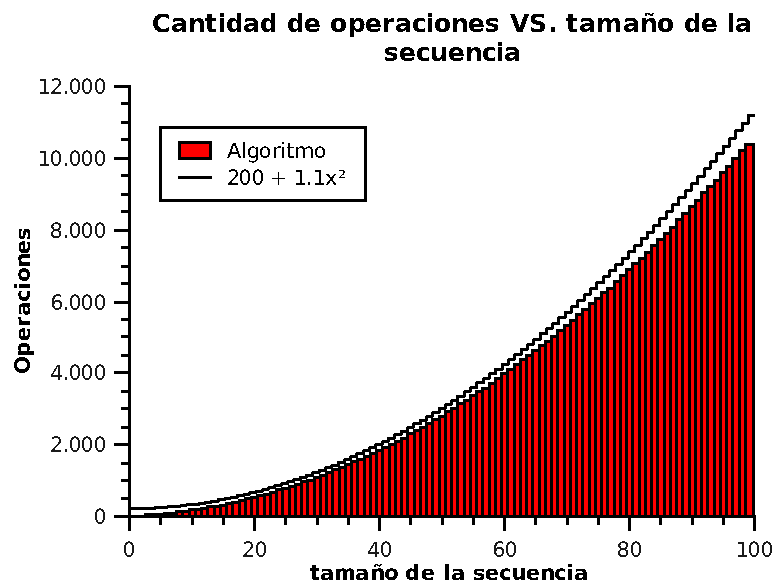
\includegraphics[scale=0.7]{../ej1/graficos/operaciones100.pdf}
				\end{tabular}
				\label{tiempoEj1a} %con esto puedo referenciar a la tabla \ref{Tiempo metodos}
	\end{table}

Estos gráficos muestran el tiempo de ejecución y cantidad de operaciones en secuencias de 1 hasta 100 elementos aleatorios comparados con funciones cuadraticas (se corresponden con la entrada generada número ``1''  de las enunciadas anteriormente).

 \vspace*{1cm}
\hspace*{-2.1cm}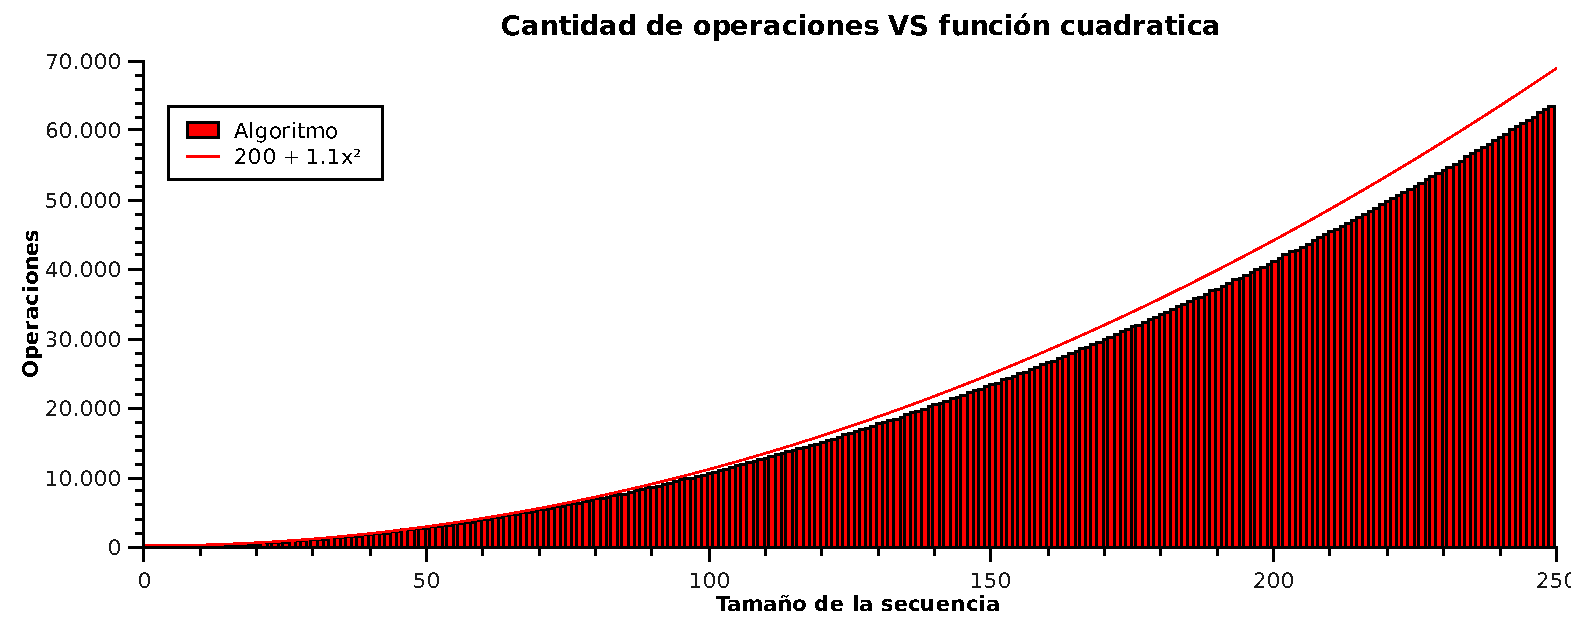
\includegraphics[width=475pt]{../ej1/graficos/operaciones250.pdf}

Este gráfico muestra la cantidad de operaciones en secuencias de 1 hasta 250 elementos aleatorios comparados con funciones cuadraticas (se corresponde con la entrada generada número ``2'' de las enunciadas anteriormente).

 \vspace*{1cm}
\hspace*{-2.1cm}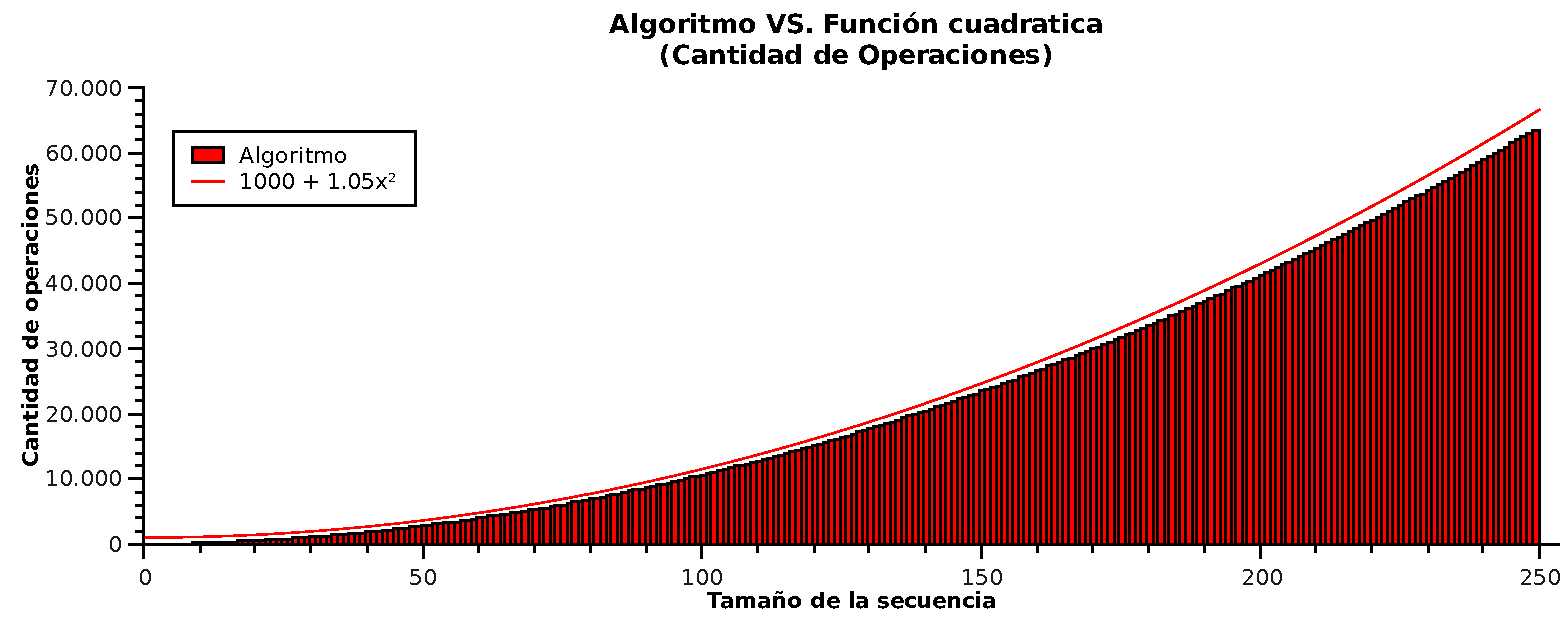
\includegraphics[width=475pt]{../ej1/graficos/operaciones0.pdf}

Este gráfico muestra la cantidad de operaciones en secuencias de 1 hasta 250 elementos iguales a cero comparados con funciones cuadraticas (se corresponde con la entrada generada número ``3'' de las enunciadas anteriormente).

 \vspace*{1cm}
\hspace*{-2.1cm}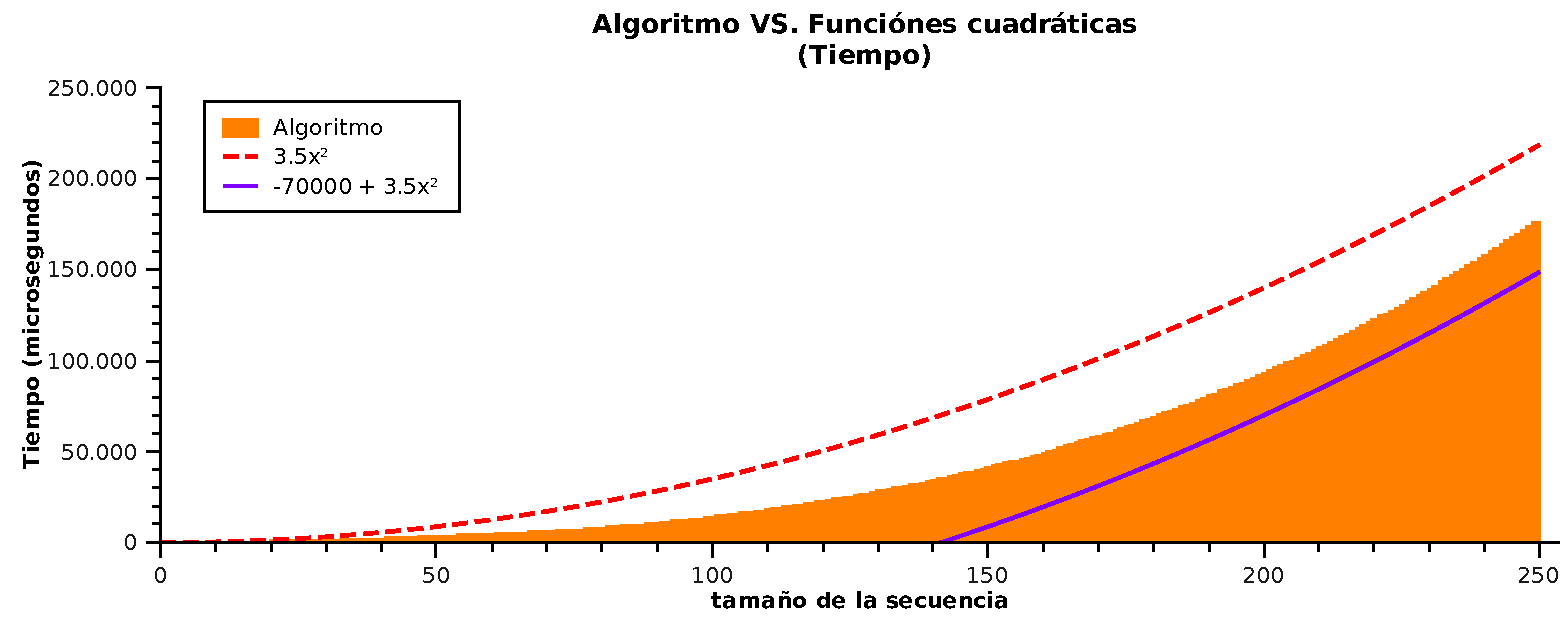
\includegraphics[width=475pt]{../ej1/graficos/tiempo0.pdf}

Este gráfico muestra la cantidad de operaciones en secuencias de 1 hasta 250 elementos comparados con funciones cuadraticas (se corresponde con la entrada generada número ``3'' de las enunciadas anteriormente).

Notar que para el mismo tipo de gráficos (de tiempo o de cantidad de operaciones), se utiliza las mismas funciónes cuadraticas para gráficar la cota superior e inferior que en el resto más alla de ser diferentes casos de pruebas. 




\subsection{Debate}
\paragraph{}
Se puede apreciar en los gráficos propuestos en la sección [\ref{resultadosej1}] que en general la implementación realizada se comporta como se esperaba que en teoría lo hiciera. Es decir, durante el desarrollo del informe sobre este ejercicio, entre otras cosas, se postuló la hipótesis de que la complejidad del algoritmo tenía un costo de $\theta(tam(v)^2)$, donde $tam(v)$ es la cantidad de números en la secuencia.

\paragraph{}
Se puede identificar en cada gráfico una marcada similitud entre los resultados arrojados en las distintas mediciones que se hicieron sobre la implementación unas parabola (o funciónes cuadráticas) cuyas pendientes no varian para cada caso (medidos de la misma manera).


\paragraph{}


\subsection{Conclusiones}
\paragraph{}
Luego de describir el funcionamiento del algoritmo, de realizar las pruebas y gráficos pertinentes y de analizarlos detalladamente, podemos realizar algunas conclusiones.\\
Podemos asegurar fehacientemente que la complejidad del algoritmo propuesto es cuadratico y que la misma es \titade{n} donde $n$ es la cantidad de trabajadores. Esto no sólo se desprende del análisis teórico realizado anteriormente, sino también de las sucesivas pruebas realizadas. Claramente se puede observar en todos los gráficos presentados cómo el comportamiento de la implementación se asemeja a una función lineal sobre los datos de entrada.

\paragraph{}
Finalmente, si hacemos una comparación entre los resultados obtenidos al aplicarse el algoritmo sobre datos de entrada azarosos y datos de entrada que se condicen con el peor caso, se puede observar que la constante que acompaña a la complejidad para el peor caso es considerablemente mayor a la constante que aparece en el caso azaroso. Como una conclusión poco menos significativa entonces, se puede decir que los casos en que los horarios de los trabajadores son todos disjuntos son los peores casos para este algoritmo.

